% Options for packages loaded elsewhere
\PassOptionsToPackage{unicode}{hyperref}
\PassOptionsToPackage{hyphens}{url}
%
\documentclass[
]{book}
\usepackage{amsmath,amssymb}
\usepackage{iftex}
\ifPDFTeX
  \usepackage[T1]{fontenc}
  \usepackage[utf8]{inputenc}
  \usepackage{textcomp} % provide euro and other symbols
\else % if luatex or xetex
  \usepackage{unicode-math} % this also loads fontspec
  \defaultfontfeatures{Scale=MatchLowercase}
  \defaultfontfeatures[\rmfamily]{Ligatures=TeX,Scale=1}
\fi
\usepackage{lmodern}
\ifPDFTeX\else
  % xetex/luatex font selection
\fi
% Use upquote if available, for straight quotes in verbatim environments
\IfFileExists{upquote.sty}{\usepackage{upquote}}{}
\IfFileExists{microtype.sty}{% use microtype if available
  \usepackage[]{microtype}
  \UseMicrotypeSet[protrusion]{basicmath} % disable protrusion for tt fonts
}{}
\makeatletter
\@ifundefined{KOMAClassName}{% if non-KOMA class
  \IfFileExists{parskip.sty}{%
    \usepackage{parskip}
  }{% else
    \setlength{\parindent}{0pt}
    \setlength{\parskip}{6pt plus 2pt minus 1pt}}
}{% if KOMA class
  \KOMAoptions{parskip=half}}
\makeatother
\usepackage{xcolor}
\usepackage{longtable,booktabs,array}
\usepackage{calc} % for calculating minipage widths
% Correct order of tables after \paragraph or \subparagraph
\usepackage{etoolbox}
\makeatletter
\patchcmd\longtable{\par}{\if@noskipsec\mbox{}\fi\par}{}{}
\makeatother
% Allow footnotes in longtable head/foot
\IfFileExists{footnotehyper.sty}{\usepackage{footnotehyper}}{\usepackage{footnote}}
\makesavenoteenv{longtable}
\usepackage{graphicx}
\makeatletter
\def\maxwidth{\ifdim\Gin@nat@width>\linewidth\linewidth\else\Gin@nat@width\fi}
\def\maxheight{\ifdim\Gin@nat@height>\textheight\textheight\else\Gin@nat@height\fi}
\makeatother
% Scale images if necessary, so that they will not overflow the page
% margins by default, and it is still possible to overwrite the defaults
% using explicit options in \includegraphics[width, height, ...]{}
\setkeys{Gin}{width=\maxwidth,height=\maxheight,keepaspectratio}
% Set default figure placement to htbp
\makeatletter
\def\fps@figure{htbp}
\makeatother
\setlength{\emergencystretch}{3em} % prevent overfull lines
\providecommand{\tightlist}{%
  \setlength{\itemsep}{0pt}\setlength{\parskip}{0pt}}
\setcounter{secnumdepth}{5}
\usepackage{booktabs}
\ifLuaTeX
  \usepackage{selnolig}  % disable illegal ligatures
\fi
\usepackage[]{natbib}
\bibliographystyle{plainnat}
\usepackage{bookmark}
\IfFileExists{xurl.sty}{\usepackage{xurl}}{} % add URL line breaks if available
\urlstyle{same}
\hypersetup{
  pdftitle={GTI - Governança da Informação - 2025 - Anotações de aula},
  pdfauthor={Professor Miguél Suares},
  hidelinks,
  pdfcreator={LaTeX via pandoc}}

\title{GTI - Governança da Informação - 2025 - Anotações de aula}
\author{Professor Miguél Suares}
\date{2025-08-23}

\begin{document}
\maketitle

{
\setcounter{tocdepth}{1}
\tableofcontents
}
\chapter*{Sobre estas anotações}\label{sobre-estas-anotauxe7uxf5es}
\addcontentsline{toc}{chapter}{Sobre estas anotações}

---------------------------------------------------------------------------------------------------------------------------------------

Estas anotações são apenas lembretes das aulas expostas em sala, durante a disciplina de Governança da Informação.

\section{ACESSO AO GITBOOK CELULAR}\label{acesso-ao-gitbook-celular}

---------------------------------------------------------------------------------------------------------------------------------------

\subsubsection{\texorpdfstring{\url{https://miguel7penteado.github.io/2025-2sem-GTI-Governanca}}{https://miguel7penteado.github.io/2025-2sem-GTI-Governanca}}\label{httpsmiguel7penteado.github.io2025-2sem-gti-governanca}


\includegraphics{images/qr-code-disciplina.jpg}

\section{Leitores de formato de arquivo EPUB para SmartPhone}\label{leitores-de-formato-de-arquivo-epub-para-smartphone}

---------------------------------------------------------------------------------------------------------------------------------------

\subsection{ANDROID}\label{android}

\subsubsection{\texorpdfstring{\textbf{Moon+ Reader}}{Moon+ Reader}}\label{moon-reader}


\includegraphics[width=3.54167in,height=\textheight]{images/qrcode/leitor_epub/MoonReaderPlus.jpg}

\section{Livros Texto da Disciplina}\label{livros-texto-da-disciplina}

---------------------------------------------------------------------------------------------------------------------------------------

\subsection{\texorpdfstring{``Governança Corporativa'' dos autores ``\textbf{José Paschoal Rossetti e Adriana Andrade}''}{``Governança Corporativa'' dos autores ``José Paschoal Rossetti e Adriana Andrade''}}\label{governanuxe7a-corporativa-dos-autores-josuxe9-paschoal-rossetti-e-adriana-andrade}


\includegraphics{images/livros/livro1.jpg}

\begin{longtable}[]{@{}
  >{\raggedright\arraybackslash}p{(\columnwidth - 2\tabcolsep) * \real{0.5000}}
  >{\raggedright\arraybackslash}p{(\columnwidth - 2\tabcolsep) * \real{0.5000}}@{}}
\toprule\noalign{}
\endhead
\bottomrule\noalign{}
\endlastfoot
\textbf{Autor(es)} & \href{https://www.fdc.org.br/sobreafdc/professores/rossetti}{\textbf{José Paschoal Rossetti}} \textbf{e \href{https://tradeconbusiness.com.br/nossa-equipe/adriana-de-andrade-sole/}{Adriana Andrade}} \\
\textbf{Editora} & Atlas \\
\textbf{Idioma} & Português \\
\textbf{ISBN} & 9788522493050 \\
\textbf{Formato} & Capa dura \\
\textbf{Páginas} & 608 \\
\textbf{Código Biblioteca} & \\
\end{longtable}

\subsection{``Implantando a Governança de TI (4ª edição): Da estratégia à gestão de processos e serviços'' dos autores ``Aguinaldo Aragon Fernandes e Vladimir Ferraz de Abreu''}\label{implantando-a-governanuxe7a-de-ti-4uxaa-ediuxe7uxe3o-da-estratuxe9gia-uxe0-gestuxe3o-de-processos-e-serviuxe7os-dos-autores-aguinaldo-aragon-fernandes-e-vladimir-ferraz-de-abreu}


\includegraphics{images/livros/livro2.jpg}

\begin{longtable}[]{@{}
  >{\raggedright\arraybackslash}p{(\columnwidth - 2\tabcolsep) * \real{0.1290}}
  >{\raggedright\arraybackslash}p{(\columnwidth - 2\tabcolsep) * \real{0.8710}}@{}}
\toprule\noalign{}
\endhead
\bottomrule\noalign{}
\endlastfoot
\textbf{Autor(es)} & \begin{minipage}[t]{\linewidth}\raggedright
\subsubsection{\texorpdfstring{\href{https://br.linkedin.com/in/aguinaldo-aragon-fernandes}{Aguinaldo Aragon Fernandes} e \href{https://br.linkedin.com/in/vladimirabreu}{Vladimir Ferraz de Abreu}}{Aguinaldo Aragon Fernandes e Vladimir Ferraz de Abreu}}\label{aguinaldo-aragon-fernandes-e-vladimir-ferraz-de-abreu}
\end{minipage} \\
\textbf{Editora} & BRASPORT \\
\textbf{Idioma} & Português \\
\textbf{ISBN-13} & 978-8574528441 \\
\textbf{Formato} & Eletrônico \\
\textbf{Páginas} & 1198 \\
\textbf{Código Biblioteca} & \\
\end{longtable}

\section{Calendário das aulas}\label{calenduxe1rio-das-aulas}

---------------------------------------------------------------------------------------------------------------------------------------

\paragraph{AGOSTO DE 2025}\label{agosto-de-2025}

\begin{longtable}[]{@{}llll@{}}
\toprule\noalign{}
Data & Dia da Semana & Aulas & Conteúdo \\
\midrule\noalign{}
\endhead
\bottomrule\noalign{}
\endlastfoot
06/08/2025 & Quarta-Feira & Aula Inaugural & \\
13/08/2025 & Quarta-Feira & Aula 2 & \\
20/08/2025 & Quarta-Feira & Aula 3 & \\
27/08/2025 & Quarta-Feira & Aula 4 & \\
\end{longtable}

\paragraph{SETEMBRO DE 2025}\label{setembro-de-2025}

\begin{longtable}[]{@{}llll@{}}
\toprule\noalign{}
Data & Dia da Semana & Aulas & Conteúdo \\
\midrule\noalign{}
\endhead
\bottomrule\noalign{}
\endlastfoot
03/09/2025 & Quarta-Feira & Aula 5 & \\
10/09/2025 & Quarta-Feira & Aula 6 & \\
17/09/2025 & Quarta-Feira & NP1 & PROVA \\
24/09/2025 & Quarta-Feira & Aula 7 & \\
\end{longtable}

\paragraph{OUTUBRO DE 2025}\label{outubro-de-2025}

\begin{longtable}[]{@{}llll@{}}
\toprule\noalign{}
Data & Dia da Semana & Aulas & Conteúdo \\
\midrule\noalign{}
\endhead
\bottomrule\noalign{}
\endlastfoot
01/10/2025 & Quarta-Feira & Aula 8 & \\
08/10/2025 & Quarta-Feira & Aula 9 & \\
15/10/2025 & Quarta-Feira & Aula 10 & \\
22/10/2025 & Quarta-Feira & Aula 11 & \\
29/10/2025 & Quarta-Feira & Aula 12 & \\
\end{longtable}

\paragraph{NOVEMBRO DE 2025}\label{novembro-de-2025}

\begin{longtable}[]{@{}llll@{}}
\toprule\noalign{}
Data & Dia da Semana & Aulas & Conteúdo \\
\midrule\noalign{}
\endhead
\bottomrule\noalign{}
\endlastfoot
05/11/2025 & Quarta-Feira & NP2 & PROVA \\
12/11/2025 & Quarta-Feira & & N/A \\
19/11/2025 & Quarta-Feira & SUB & PROVA \\
26/11/2025 & Quarta-Feira & & N/A \\
\end{longtable}

\paragraph{DEZEMBRO DE 2025}\label{dezembro-de-2025}

\begin{longtable}[]{@{}llll@{}}
\toprule\noalign{}
Data & Dia da Semana & Aulas & Conteúdo \\
\midrule\noalign{}
\endhead
\bottomrule\noalign{}
\endlastfoot
03/12/2025 & Quarta-Feira & & N/A \\
10/12/2025 & Quarta-Feira & EXAME & PROVA \\
17/12/2025 & Quarta-Feira & & N/A \\
24/12/2025 & Quarta-Feira & & NATAL \\
31/12/2025 & Quarta-Feira & & Confrat \\
\end{longtable}

\section{Alunos 2025 - 2o Semestre}\label{alunos-2025---2o-semestre}

---------------------------------------------------------------------------------------------------------------------------------------

\subsection{Campus Chácara Santo Antônio}\label{campus-chuxe1cara-santo-antuxf4nio}

\subsubsection{Turma TI3P40}\label{turma-ti3p40}

\begin{longtable}[]{@{}cc@{}}
\toprule\noalign{}
Matrícula & Nome do aluno \\
\midrule\noalign{}
\endhead
\bottomrule\noalign{}
\endlastfoot
R191BJ3 & ANDRESSA MARIA DA SILVA \\
R194GF6 & JOÃO VICTOR DE JESUS ANDRADE \\
R1704D1 & PALOMA FERNANDES D GERALDO \\
G7946I4 & VINICIUS ALMEIDA SILVA \\
\end{longtable}

\subsubsection{Turma TI4P40}\label{turma-ti4p40}

\begin{longtable}[]{@{}cc@{}}
\toprule\noalign{}
Matrícula & Nome do aluno \\
\midrule\noalign{}
\endhead
\bottomrule\noalign{}
\endlastfoot
G958DB5 & AGATHA CALUCIO SANTIAGO \\
G03IJD7 & ALESSANDRA ALMEIDA RIBEIRO \\
G993FJ5 & ANNA BEATRIZ TEIXEIRA SILVA \\
G9699B3 & CAMILA VICTORIA DE SOUZA SANTO \\
G9787H7 & LEONARDO GONCALVES R FONSECA \\
G978JB0 & LIRIEL CHAIANE M OLIVEIRA \\
R0958I0 & RENAN HENRIQUE SILVA \\
G94GFD1 & VANESSA ALMEIDA SANTOS \\
G833EG6 & WESLEY PEREIRA DOS S DE SOUSA \\
\end{longtable}

\subsection{Campus Marquês de São Vicente}\label{campus-marquuxeas-de-suxe3o-vicente}

\subsubsection{Turma TI3P13}\label{turma-ti3p13}

\begin{longtable}[]{@{}cc@{}}
\toprule\noalign{}
Matrícula & Nome do aluno \\
\midrule\noalign{}
\endhead
\bottomrule\noalign{}
\endlastfoot
F35GAE8 & LUCAS SOUZA XAVIER \\
\end{longtable}

\subsubsection{Turma TI4P13}\label{turma-ti4p13}

\begin{longtable}[]{@{}cc@{}}
\toprule\noalign{}
Matrícula & Nome do aluno \\
\midrule\noalign{}
\endhead
\bottomrule\noalign{}
\endlastfoot
F358542 & ANA JULIA DE O BARBOSA \\
R0416B5 & CAUA MARTINS SILVESTRE \\
F359549 & ERICA CALO SANTOS \\
R063HI0 & FERNANDO ROCHA QUINHOLI \\
F359573 & GABRIEL HENRIQUE M TEIXEIRA \\
R057BD6 & GUILHERME JACOB M DE MACEDO \\
G960CJ8 & GUILHERME RENATO R DE QUEIROZ \\
G978099 & ISABELA SASS MARTINS DE SOUZA \\
F3591B9 & JOAO VITOR SILVA SOUZA \\
G907582 & KAROLINE VIEIRA ARAGAO \\
\end{longtable}

\chapter{Aula Inaugural}\label{aula-inaugural}

\subsubsection*{05/08/2025 - Campus Marquês}\label{campus-marquuxeas}
\addcontentsline{toc}{subsubsection}{05/08/2025 - Campus Marquês}

\subsubsection*{06/08/2025 - Campus Chácara}\label{campus-chuxe1cara}
\addcontentsline{toc}{subsubsection}{06/08/2025 - Campus Chácara}

\subsubsection*{Professor Miguél Suares}\label{professor-miguuxe9l-suares}
\addcontentsline{toc}{subsubsection}{Professor Miguél Suares}

\section{\texorpdfstring{Disciplina: \textbf{Governança da Informação}}{Disciplina: Governança da Informação}}\label{disciplina-governanuxe7a-da-informauxe7uxe3o}

\begin{itemize}
\tightlist
\item
  Curso: Gestão em Tecnologia da Informação (GTI)\\
\item
  Período: \textbf{Noturno}\\
\item
  Turma: \textbf{4º semestre de 2025}
\item
  Campus: \textbf{Chácara Santo Antônio}
\item
  Campus: \textbf{Chácara Marquês de São Vicente}
\end{itemize}

\begin{quote}
``\emph{Reunir-se é um começo; manter-se unido é progresso; trabalhar em conjunto é sucesso.}'' --- Henry Ford
\end{quote}


\includegraphics[width=3.64583in,height=\textheight]{images/Bem_Vindo.jpg}

\begin{center}\rule{0.5\linewidth}{0.5pt}\end{center}

\section{👨‍🏫 Sobre o Professor}\label{sobre-o-professor}

\begin{itemize}
\item
  Nome: Prof.~Miguél Suares
\item
  Formação: Mestre em Engenharia da Computação e Energia da Agricultura
\item
  Experiência: +13 anos trabalhando e lidando com compliance de TIC no setor público
\item
  Contato: \href{mailto:miguel.penteado@docente.unip.br}{\nolinkurl{miguel.penteado@docente.unip.br}}
\end{itemize}

\begin{center}\rule{0.5\linewidth}{0.5pt}\end{center}

\section{🎯 Objetivos da Disciplina}\label{objetivos-da-disciplina}

\begin{itemize}
\item
  Começar compreendendo os fundamentos de Govarenança Corporativa
\item
  Compreender modelos de governança de cada área chave da empresa
\item
  Governança de TIC - Conhecer o COBIT 5.0 - certificação e Prova
\item
  Governança de TIC - Conhecer o COBIT 5.0 - Princípios e Habilitadores
\item
  Governança de TIC - Conhecer o COBIT 2019 - mudanças em relação a versão 5.0

  \includegraphics[width=3.47917in,height=\textheight]{images/2025-08-04/logos.jpg}
\end{itemize}

\begin{center}\rule{0.5\linewidth}{0.5pt}\end{center}

\section{📅 Calendário da Disciplina - Campus Marquês de São Vicente}\label{calenduxe1rio-da-disciplina---campus-marquuxeas-de-suxe3o-vicente}

\begin{longtable}[]{@{}lll@{}}
\toprule\noalign{}
Data & Aula & Tema \\
\midrule\noalign{}
\endhead
\bottomrule\noalign{}
\endlastfoot
05/08/2025 & Aula 1 & Aula Inaugural \\
12/08/2025 & Aula 2 & O topo da Pirâmide \\
19/08/2025 & Aula 3 & Assembléia dos Proprietários \\
26/08/2025 & Aula 4 & Conselhos da Empresa \\
02/09/2025 & Aula 5 & C Level e Diretorias \\
09/09/2025 & Aula 6 & Diretoria de Informática \\
16/09/2025 & \textbf{NP1} & \textbf{Prova} \\
23/09/2025 & Aula 7 & Modelo COBIT 5.0 \\
30/09/2025 & Aula 8 & COBIT 5.0 - Os 5 Princípios \\
07/10/2025 & Aula 9 & COBIT 5.0 - Os 7 Habilitadores \\
14/10/2025 & Aula 10 & COBIT 5.0 - Implantação \\
21/10/2025 & Aula 11 & COBIT 2019 - O que mudou em relação ao 5.0 \\
28/10/2025 & Aula 12 & Revisão \\
04/11/2025 & \textbf{NP2} & \textbf{Prova} \\
\end{longtable}

\begin{center}\rule{0.5\linewidth}{0.5pt}\end{center}

\section{📅 Calendário da Disciplina - Campus Chácara Santo Antônio}\label{calenduxe1rio-da-disciplina---campus-chuxe1cara-santo-antuxf4nio}

\begin{longtable}[]{@{}lll@{}}
\toprule\noalign{}
Data & Aula & Tema \\
\midrule\noalign{}
\endhead
\bottomrule\noalign{}
\endlastfoot
06/08/2025 & Aula 1 & Aula Inaugural \\
13/08/2025 & Aula 2 & O topo da Pirâmide \\
20/08/2025 & Aula 3 & Assembléia dos Proprietários \\
27/08/2025 & Aula 4 & Conselhos da Empresa \\
03/09/2025 & Aula 5 & C Level e Diretorias \\
10/09/2025 & Aula 6 & Diretoria de Informática \\
17/09/2025 & \textbf{NP1} & \textbf{Prova} \\
24/09/2025 & Aula 7 & Modelo COBIT 5.0 \\
01/10/2025 & Aula 8 & COBIT 5.0 - Os 5 Princípios \\
08/10/2025 & Aula 9 & COBIT 5.0 - Os 7 Habilitadores \\
15/10/2025 & Aula 10 & COBIT 5.0 - Implantação \\
22/10/2025 & Aula 11 & COBIT 2019 - O que mudou em relação ao 5.0 \\
29/10/2025 & Aula 12 & Revisão \\
05/11/2025 & \textbf{NP2} & \textbf{Prova} \\
\end{longtable}

\begin{center}\rule{0.5\linewidth}{0.5pt}\end{center}

\section{📚 Ementa Resumida}\label{ementa-resumida}

\begin{itemize}
\item
  Conhecer a Governança na Empresa
\item
  Conhecer a Governança de T.I.
\item
  Conhecer o Modelo COBIT 5.0
\item
  Vislumbrar o modelo COBIT 2019

  \includegraphics[width=3.44792in,height=\textheight]{images/2025-08-04/modelagem.jpg}
\end{itemize}

\begin{center}\rule{0.5\linewidth}{0.5pt}\end{center}

\section{📝 Avaliação}\label{avaliauxe7uxe3o}

\begin{itemize}
\tightlist
\item
  \textbf{Provas (NP1 + NP2)}
\item
  \textbf{Prova Substitutiva}
\item
  \textbf{Exame}
\end{itemize}

\begin{center}\rule{0.5\linewidth}{0.5pt}\end{center}

\section{🛠️ Ferramentas da Disciplina}\label{ferramentas-da-disciplina}

\begin{itemize}
\item
  Livro texto:
\item
  Questionários
\item
  Vídeos Youtube
\end{itemize}

\begin{center}\rule{0.5\linewidth}{0.5pt}\end{center}

\section{📌 Expectativas e Regras}\label{expectativas-e-regras}

\begin{itemize}
\tightlist
\item
  Pontualidade e entrega de atividades no prazo
\item
  Trabalhos devem ser originais (sem plágio)
\item
  Participação ativa nas discussões e práticas
\item
  Uso responsável das ferramentas
\item
  Respeito e colaboração entre colegas
\end{itemize}

\begin{center}\rule{0.5\linewidth}{0.5pt}\end{center}

\section{💡 Dicas para Mandar Bem}\label{dicas-para-mandar-bem}

\begin{itemize}
\tightlist
\item
  Faça os exercícios logo após a aula
\item
  Participe das práticas com base real
\end{itemize}

\begin{center}\rule{0.5\linewidth}{0.5pt}\end{center}

\section{🙌 Encerramento}\label{encerramento}

\section{Estamos prontos?}\label{estamos-prontos}

📧 Dúvidas? Estou à disposição\\
📊 Vamos construir conhecimento juntos!

\begin{quote}
Próxima aula: \textbf{Governança da Informação} -- 11/08/2025
\end{quote}

\chapter{Governança Corporativa - O topo da Pirâmide}\label{governanuxe7a-corporativa---o-topo-da-piruxe2mide}

\subsubsection*{12/08/2025 - Campus Marquês}\label{campus-marquuxeas-1}
\addcontentsline{toc}{subsubsection}{12/08/2025 - Campus Marquês}

\subsubsection*{13/08/2025 - Campus Chácara}\label{campus-chuxe1cara-1}
\addcontentsline{toc}{subsubsection}{13/08/2025 - Campus Chácara}

\begin{center}\rule{0.5\linewidth}{0.5pt}\end{center}

\section{O que é Governança Corporativa}\label{o-que-uxe9-governanuxe7a-corporativa}

No livro ``Governança Corporativa'', os autores \textbf{José Paschoal Rossetti e Adriana Andrade} dão a seguinte definição para Governaça Corporativa:

\begin{quote}
\textbf{Um sistema pelo qual as sociedades empresárias são dirigidas e monitoradas, envolvendo os relacionamentos entre sócios/cotistas, conselho de administração, diretoria, auditoria independente e conselho fiscal. -} \emph{Rossetti e Andrade -}
\end{quote}

a

\section{Quais motivos criam a necessidade de Governança Corporativa ?}\label{quais-motivos-criam-a-necessidade-de-governanuxe7a-corporativa}

\begin{itemize}
\tightlist
\item
  Quantidade de funcionários da empresa ?
\item
  Tamanho da corporação ?
\item
  Ramo de atividade da empresa ?
\item
  Faturamento mensal/anual da empresa ?
\end{itemize}


\includegraphics[width=2.69792in,height=\textheight]{images/02-2025-08-12_13/01-Ale_costa_Cacau_Show.jpg} \textbar{} 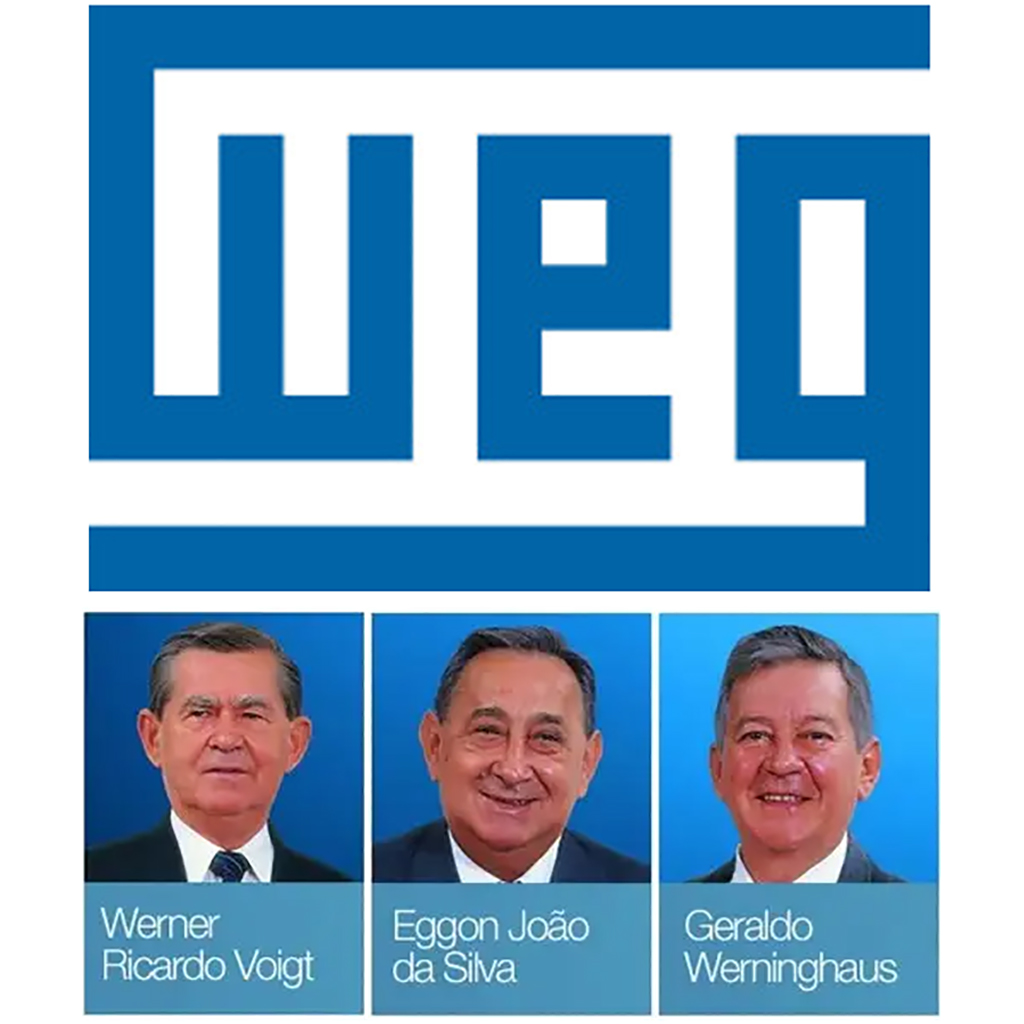
\includegraphics[width=1.27083in,height=\textheight]{images/02-2025-08-12_13/02-Weg.jpg}

\begin{center}\rule{0.5\linewidth}{0.5pt}\end{center}

\section{O principal fator é o número efetivo ou potencial de sócios}\label{o-principal-fator-uxe9-o-nuxfamero-efetivo-ou-potencial-de-suxf3cios}

\begin{itemize}
\tightlist
\item
  \textbf{Efetivo:} NÚMERO DE SÓCIOS
\end{itemize}

\begin{longtable}[]{@{}
  >{\centering\arraybackslash}p{(\columnwidth - 2\tabcolsep) * \real{0.4722}}
  >{\raggedright\arraybackslash}p{(\columnwidth - 2\tabcolsep) * \real{0.5278}}@{}}
\toprule\noalign{}
\begin{minipage}[b]{\linewidth}\centering
EFETIVO CASO DE GRANDE NÚMERO DE SÓCIOS
\end{minipage} & \begin{minipage}[b]{\linewidth}\raggedright
\end{minipage} \\
\midrule\noalign{}
\endhead
\bottomrule\noalign{}
\endlastfoot
\textbf{\emph{EMPRESA S/A (CAPITAL ABERTO)}} & 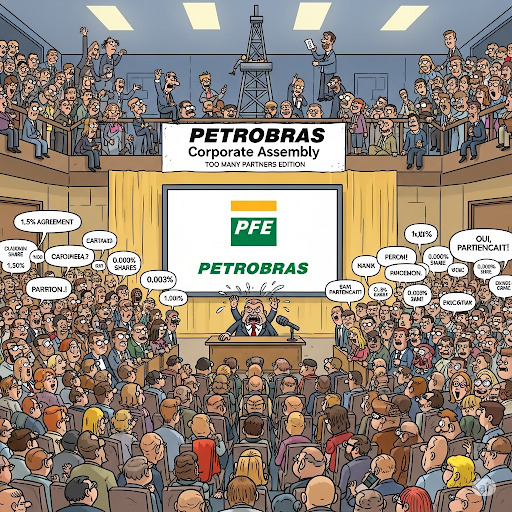
\includegraphics{images/02-2025-08-12_13/00-PetroBras.jpg} \\
\end{longtable}

\begin{center}\rule{0.5\linewidth}{0.5pt}\end{center}

\section{O principal fator é o número efetivo ou potencial de sócios}\label{o-principal-fator-uxe9-o-nuxfamero-efetivo-ou-potencial-de-suxf3cios-1}

\begin{itemize}
\item
  \textbf{Potencial:} futuro número de sócios !

  \begin{longtable}[]{@{}
    >{\centering\arraybackslash}p{(\columnwidth - 2\tabcolsep) * \real{0.3611}}
    >{\centering\arraybackslash}p{(\columnwidth - 2\tabcolsep) * \real{0.6389}}@{}}
  \toprule\noalign{}
  \begin{minipage}[b]{\linewidth}\centering
  POTENCIAL CASO DE AUMENTO DE SÓCIOS
  \end{minipage} & \begin{minipage}[b]{\linewidth}\centering
  \end{minipage} \\
  \midrule\noalign{}
  \endhead
  \bottomrule\noalign{}
  \endlastfoot
  \textbf{FUSÕES} & 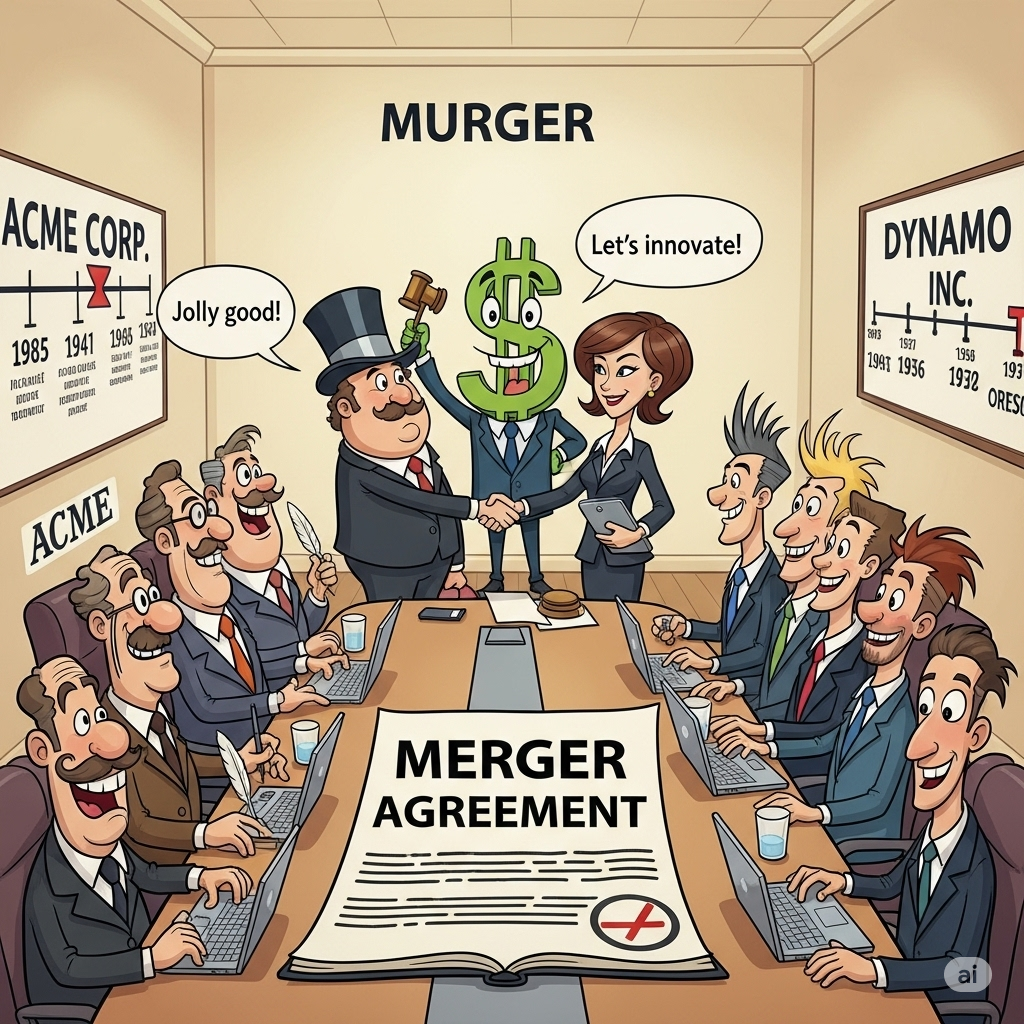
\includegraphics[width=2.46875in,height=\textheight]{images/02-2025-08-12_13/04-Fusao_Corporativa.jpg} \\
  \textbf{AQUISIÇÕES} & \\
  \textbf{INCORPORAÇÕES} & \\
  \textbf{SUCESSÃO FAMILIAR} & \includegraphics[width=1.95833in,height=\textheight]{images/02-2025-08-12_13/03-sucessao_familiar.jpg} \\
  \end{longtable}
\end{itemize}

\begin{center}\rule{0.5\linewidth}{0.5pt}\end{center}

\section{Casos que normalmente demandam arquitetura de governança corporativa}\label{casos-que-normalmente-demandam-arquitetura-de-governanuxe7a-corporativa}

\begin{itemize}
\item
  Sucessão familiar que amplie significativamente o número de sócios\\
  \emph{(filhos -- 1ª geração --, netos -- 2ª geração -- etc.)}

  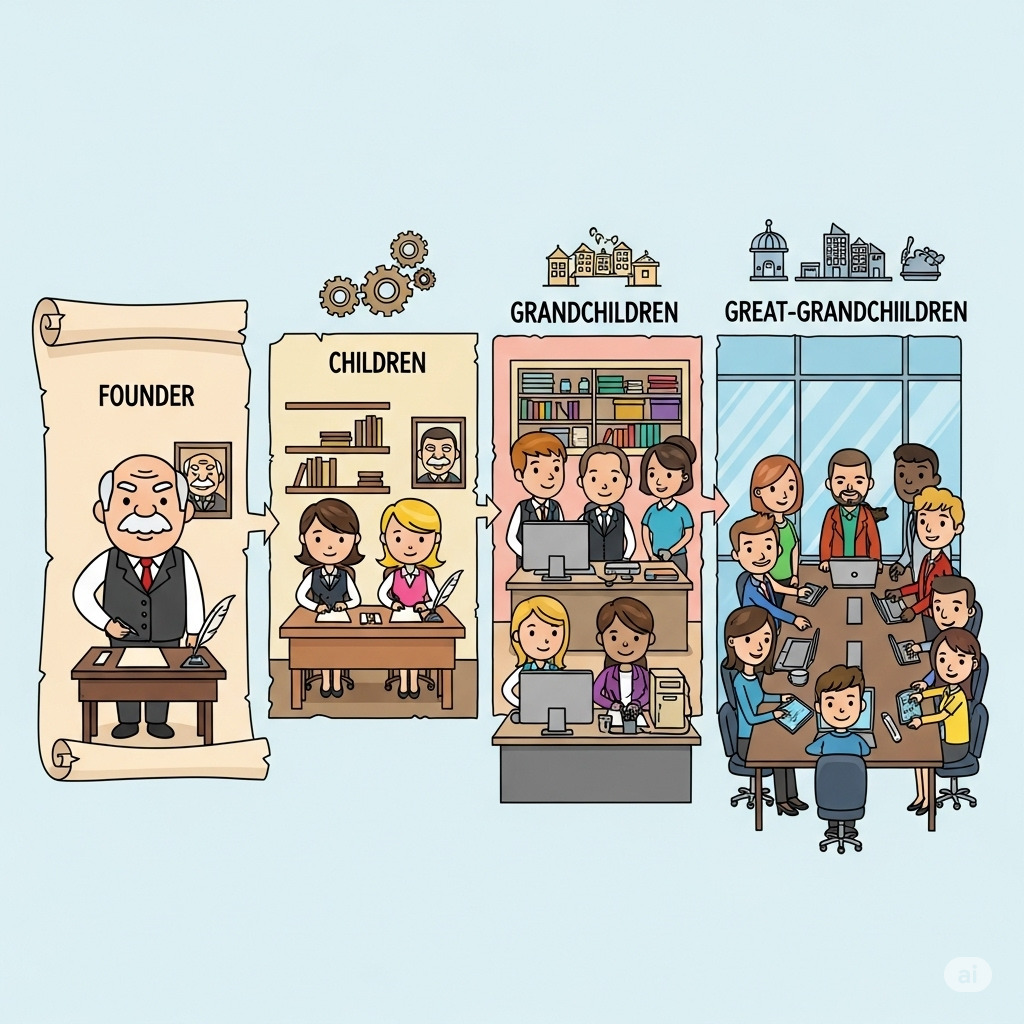
\includegraphics[width=5.69792in,height=\textheight]{images/02-2025-08-12_13/05-linha_sucessoria.jpg}
\item
  Fusão ou incorporação que amplie o número de acionistas ou cotistas
\item
  Sociedade que já nasça com grande número de acionistas ou cotistas
\end{itemize}

\begin{center}\rule{0.5\linewidth}{0.5pt}\end{center}

\section{Arquitetura de Governança}\label{arquitetura-de-governanuxe7a}

\begin{itemize}
\item
  Topo - Assembléia de Acionistas/Cotistas
\item
  2o Degrau - Conselhos (Administrativo, Fiscal e Consultivo)
\item
  3o Degrau - CEO
\item
  4o Degrau - Diretorias
\end{itemize}

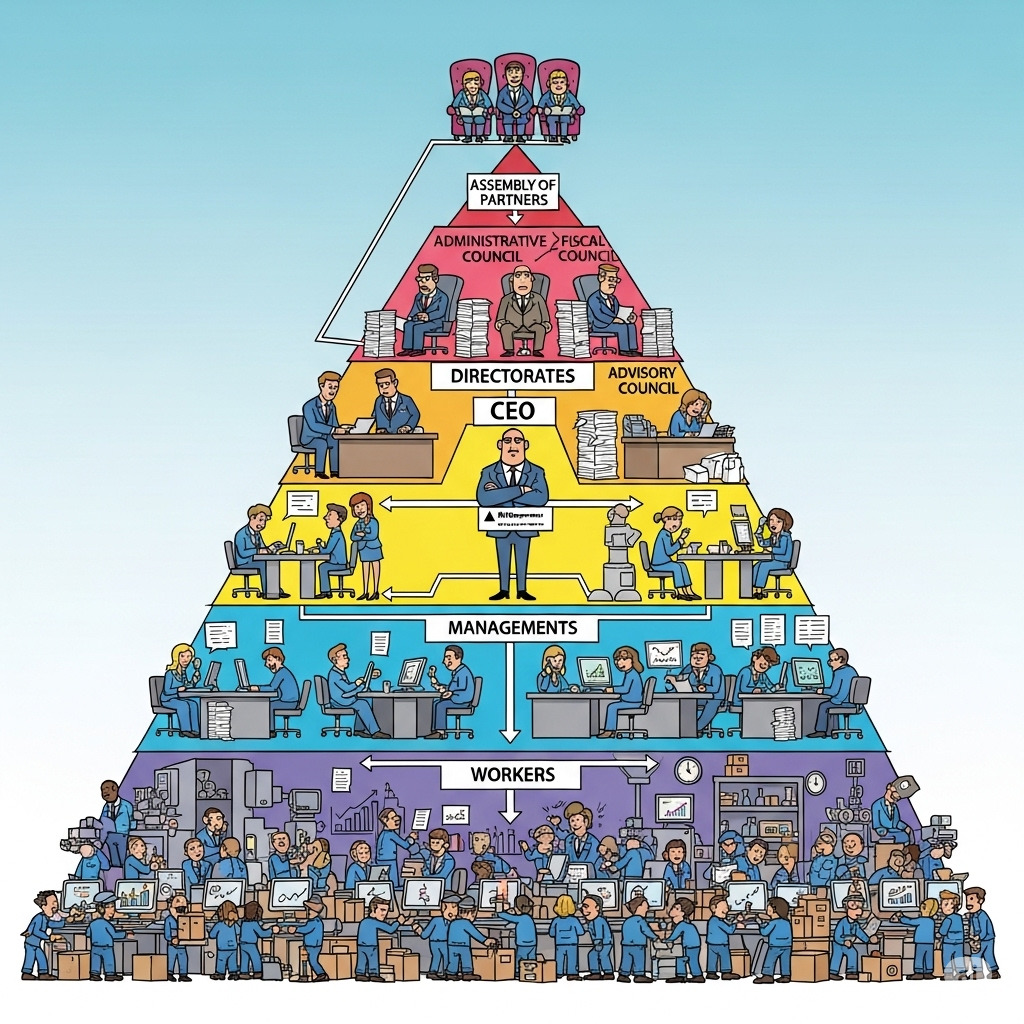
\includegraphics{images/02-2025-08-12_13/00-topo_piramide.jpg}

\begin{center}\rule{0.5\linewidth}{0.5pt}\end{center}

\subsection{ARQUÉTIPOS de Governança Corporativa}\label{arquuxe9tipos-de-governanuxe7a-corporativa}

\begin{itemize}
\item
  \textbf{SEPARAÇÃO DE PROPRIEDADE E GESTÃO}
\item
  Anglo-Saxão
\item
  Alemão
\item
  Francês
\item
  Japonês
\item
  Latino-Americano
\end{itemize}

\begin{center}\rule{0.5\linewidth}{0.5pt}\end{center}

\subsubsection{Modelo Anglo-Saxão de Governança Corporativa}\label{modelo-anglo-saxuxe3o-de-governanuxe7a-corporativa}


\includegraphics[width=1.48958in,height=\textheight]{images/02-2025-08-12_13/06-modelo_anglo-saxao.jpg}

\subsection{Características definidoras}\label{caracteruxedsticas-definidoras}

\textbf{Financiamento predominante} - Fonte principal: mercado de capitais - Ações (equity) como base da capitalização - Fundos de pensão com grande parte do patrimônio em ações - Orientação para o mercado

\textbf{Propriedade e controle acionário} - Estrutura patrimonial pulverizada - Raros acionistas com mais de 10\% do capital nas maiores empresas

\textbf{Propriedade e gestão} - Dissociação entre propriedade e gestão

\textbf{Conflitos de agência} - Principal conflito: acionistas x gestores - Altos custos de agência

\textbf{Proteção legal a minoritários} - Forte, por leis e regulação do mercado

\begin{center}\rule{0.5\linewidth}{0.5pt}\end{center}

\subsubsection{Modelo Alemão de Governança Corporativa}\label{modelo-alemuxe3o-de-governanuxe7a-corporativa}


\includegraphics[width=2.34375in,height=\textheight]{images/02-2025-08-12_13/07-modelo_alemao.jpg}

\subsection{Características definidoras}\label{caracteruxedsticas-definidoras-1}

\textbf{Financiamento predominante} - Crédito bancário de longo prazo como principal fonte - Relação duradoura com bancos, reduzindo assimetria de informação

\textbf{Propriedade e controle acionário} - Estrutura patrimonial concentrada - Bancos e grandes acionistas controlam boa parte do capital

\textbf{Propriedade e gestão} - Bancos com grande poder, monitorando interesses dos credores

\textbf{Conflitos de agência} - Principal risco: expropriação de minoritários - Conflitos caros são raros

\textbf{Proteção legal a minoritários} - Não é prioridade; tendência de fortalecer o mercado de ações

\begin{center}\rule{0.5\linewidth}{0.5pt}\end{center}

\subsubsection{Modelo Japonês de Governança Corporativa}\label{modelo-japonuxeas-de-governanuxe7a-corporativa}


\includegraphics[width=2.13542in,height=\textheight]{images/02-2025-08-12_13/09-modelo_japones.jpg}

\subsection{Características definidoras}\label{caracteruxedsticas-definidoras-2}

\textbf{Financiamento predominante} - Bancos financiam via dívida de longo prazo - Relação duradoura entre bancos e empresas

\textbf{Propriedade e controle acionário} - Concentração peculiar: keiretsu com posse cruzada de ações

\textbf{Propriedade e gestão} - Sobreposição; predominância do consenso

\textbf{Conflitos de agência} - Custos e conflitos insignificantes

\textbf{Proteção legal a minoritários} - Sustentação de relações de longo prazo - Gestão voltada a múltiplos interesses

\begin{center}\rule{0.5\linewidth}{0.5pt}\end{center}

\subsubsection{Modelo Francês de Governança Corporativa}\label{modelo-francuxeas-de-governanuxe7a-corporativa}


\includegraphics[width=2.0625in,height=\textheight]{images/02-2025-08-12_13/08-modelo_frances.jpg}

\subsection{Características definidoras}\label{caracteruxedsticas-definidoras-3}

\textbf{Financiamento predominante} - Indefinido, mas alavancagem relevante - Forte presença de empresas familiares fechadas

\textbf{Propriedade e controle acionário} - Controle concentrado

\textbf{Propriedade e gestão} - Sobreposição; gestão fechada - Conselhos com função mais consultiva

\textbf{Conflitos de agência} - Baixos conflitos devido à concentração - Risco de expropriação de minoritários

\textbf{Proteção legal a minoritários} - Fraca, com baixo enforcement - Mercados de capitais pouco desenvolvidos

\begin{center}\rule{0.5\linewidth}{0.5pt}\end{center}

\subsubsection{Modelo Latino-Americano de Governança Corporativa}\label{modelo-latino-americano-de-governanuxe7a-corporativa}


\includegraphics[width=3.1875in,height=\textheight]{images/02-2025-08-12_13/10-modelo_latino_americano.jpg}

\subsection{Características definidoras}\label{caracteruxedsticas-definidoras-4}

\textbf{Financiamento predominante} - Predomínio da dívida - Mercados de capitais pouco expressivos

\textbf{Propriedade e controle acionário} - Propriedade concentrada - Maior participação estrangeira nos últimos anos

\textbf{Propriedade e gestão} - Exercida pelos majoritários

\textbf{Conflitos de agência} - Entre acionistas majoritários e minoritários

\textbf{Proteção legal a minoritários} - Predominantemente fraca - Alta proporção de ações sem voto

\section{Referências}\label{referuxeancias}

ROSSETTI, José Paschoal; ANDRADE, Adriana. \emph{Governança Corporativa: Fundamentos, Desenvolvimento e Tendências}. São Paulo: Atlas, 7. ed., 2014. p.~s.p.

\begin{center}\rule{0.5\linewidth}{0.5pt}\end{center}

\chapter{Governança Corporativa - Assembléia dos Proprietários}\label{governanuxe7a-corporativa---assembluxe9ia-dos-proprietuxe1rios}

\subsubsection*{19/08/2025 - Campus Marquês}\label{campus-marquuxeas-2}
\addcontentsline{toc}{subsubsection}{19/08/2025 - Campus Marquês}

\subsubsection*{20/08/2025 - Campus Chácara}\label{campus-chuxe1cara-2}
\addcontentsline{toc}{subsubsection}{20/08/2025 - Campus Chácara}

\subsection{Livro ``Governança Corporativa''}\label{livro-governanuxe7a-corporativa}

\subsubsection{capítulo ``A Assembleia Geral no processo de governança'', pág 267}\label{capuxedtulo-a-assembleia-geral-no-processo-de-governanuxe7a-puxe1g-267}

\section{\texorpdfstring{\textbf{A Assembleia Geral}}{A Assembleia Geral}}\label{a-assembleia-geral}

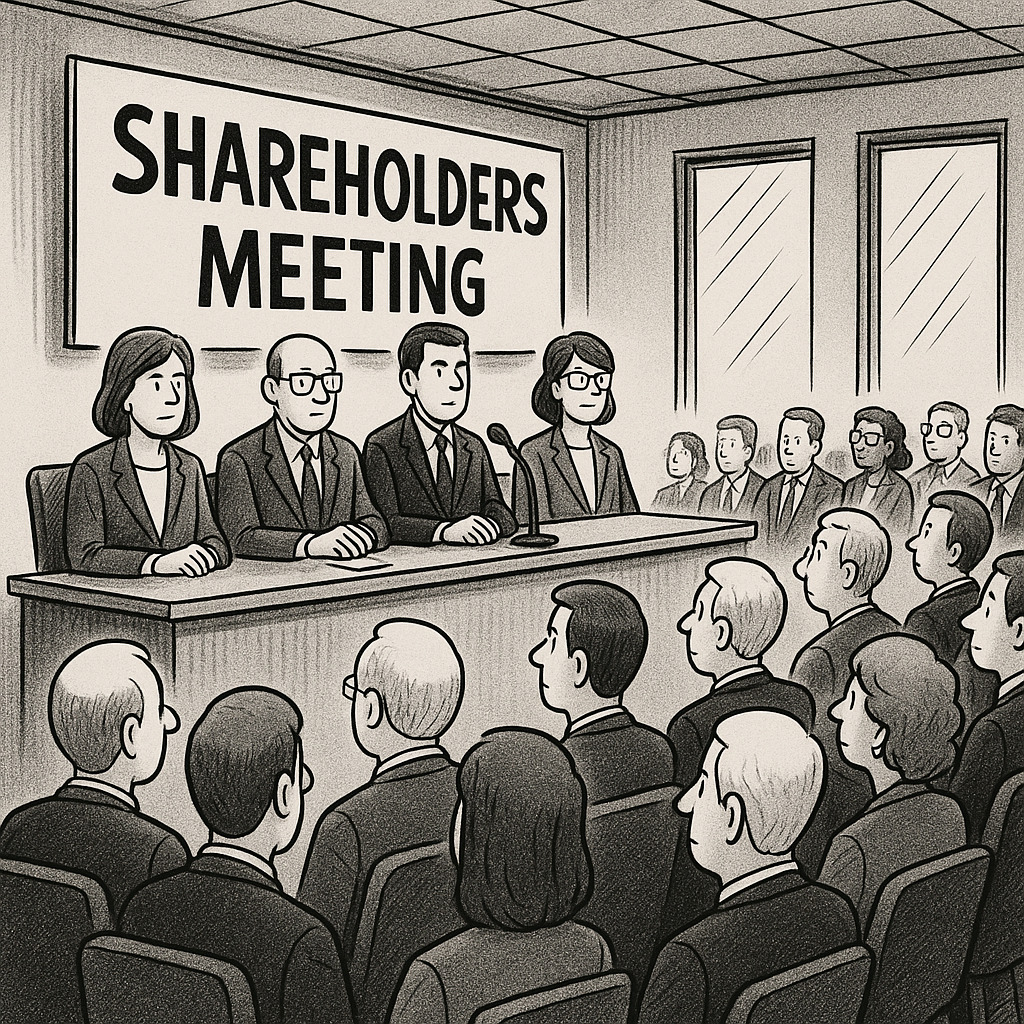
\includegraphics[width=5.36458in,height=\textheight]{images/03-2025-08-19_20/01-assembleia_cotistas.jpg}

É definida como a \textbf{reunião de acionistas ou cotistas}.

É considerada o \textbf{órgão soberano da organização}.

\section{\texorpdfstring{\textbf{Principais Competências da Assembleia Geral}}{Principais Competências da Assembleia Geral}}\label{principais-competuxeancias-da-assembleia-geral}

As competências destacadas da Assembleia Geral incluem:

\begin{itemize}
\item
  \textbf{Aumentar ou reduzir o capital social} e \textbf{reformar o estatuto/contrato social}.
\item
  \textbf{Eleger ou destituir}, a qualquer tempo, \textbf{conselheiros de administração e fiscais}.
\item
  Tomar, anualmente, as \textbf{contas dos administradores} e deliberar sobre as \textbf{demonstrações financeiras}.
\item
  Deliberar sobre \textbf{transformação, fusão, incorporação, cisão, dissolução e liquidação da sociedade}.
\item
  Deliberar sobre a \textbf{avaliação de bens} que venham a integralizar o capital social.
\item
  \textbf{Aprovar a remuneração dos administradores}.
\end{itemize}

\section{\texorpdfstring{\textbf{Frequência e Modalidade das Assembleias}}{Frequência e Modalidade das Assembleias}}\label{frequuxeancia-e-modalidade-das-assembleias}

A Assembleia Geral pode ser de dois tipos, elecandos abaixo:

\subsection{\texorpdfstring{\textbf{Assembleia Geral Ordinária (AGO)}}{Assembleia Geral Ordinária (AGO)}}\label{assembleia-geral-ordinuxe1ria-ago}

Ocorre uma vez por ano com o objetivo de \textbf{aprovar as contas do exercício e o planejamento do ano seguinte}.

\subsection{\texorpdfstring{\textbf{Assembleia Geral Extraordinária (AGE)}}{Assembleia Geral Extraordinária (AGE)}}\label{assembleia-geral-extraordinuxe1ria-age}

Pode ocorrer a qualquer momento, \textbf{sendo convocada por administradores ou acionistas/cotistas}, de acordo com as regras previstas no estatuto social.

\section{Participação Patromonial na empresa (Equity)}\label{participauxe7uxe3o-patromonial-na-empresa-equity}

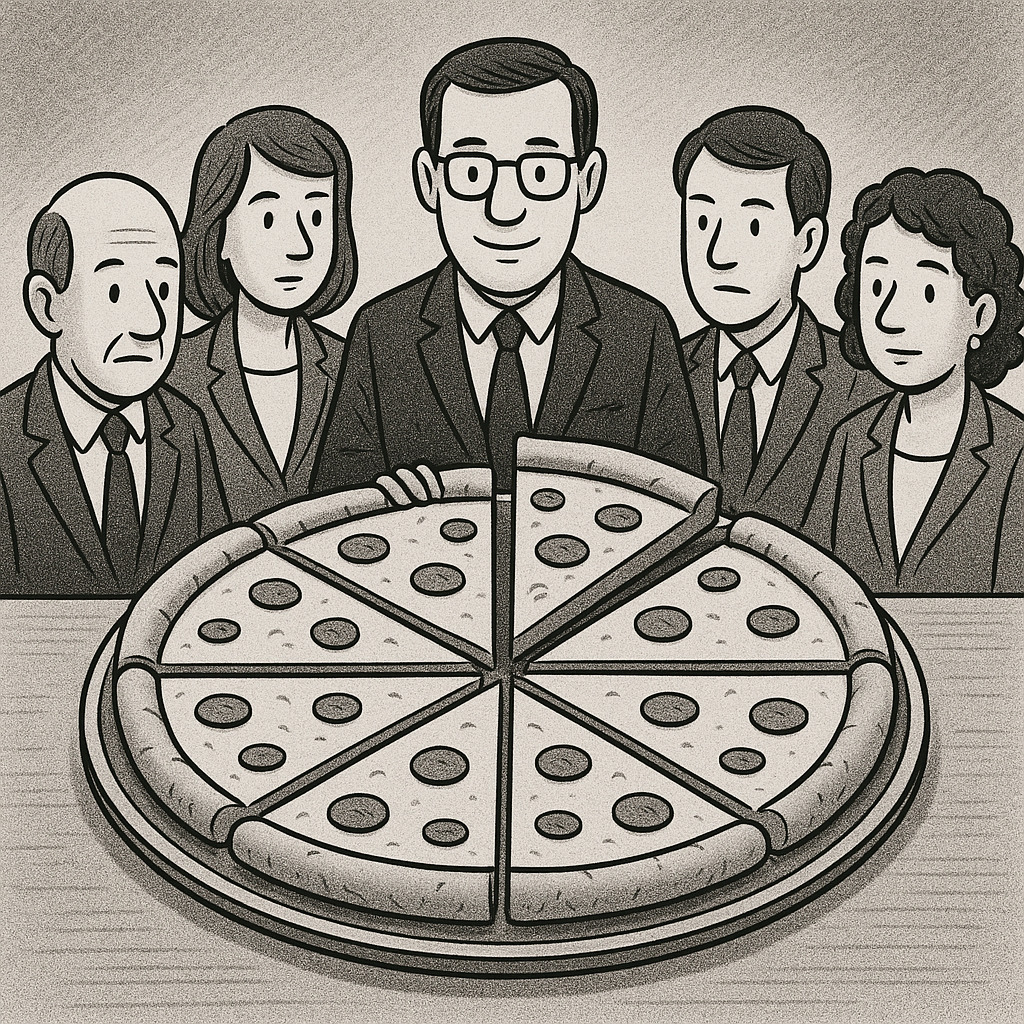
\includegraphics[width=2.3125in,height=\textheight]{images/03-2025-08-19_20/02-assembleia_cotistas-equity.jpg}

\subsubsection{Como calcular EQUITY após uma rodada de investimentos}\label{como-calcular-equity-apuxf3s-uma-rodada-de-investimentos}

Como um acionista pode calcular sua participação na empresa após uma rodada de investimentos ?

Basicamente, podemos fazer-lo aplicado a fórmula:

\subsubsection{Participação percentual do sócio pós-seção de participação ao investidor}\label{participauxe7uxe3o-percentual-do-suxf3cio-puxf3s-seuxe7uxe3o-de-participauxe7uxe3o-ao-investidor}

\[
Porcentagem\_Participacao\_Sócio\_Pós\_Investimento = \frac{Porcentagem\_Participacao\_Pré\_Investimento}{(1 - Participacao\_Percentual\_Investidor)}
\]

\subsubsection{Participação percentual do investidor pós-investimento monetário}\label{participauxe7uxe3o-percentual-do-investidor-puxf3s-investimento-monetuxe1rio}

\[
Participação\_Percentual\_\_Investidor = (\frac{ Dinheiro\_Investido}{ CapitalSocial\_Pós\_Investimento}) * 100%
\]

\section{Equity - caso FACEBOOK}\label{equity---caso-facebook}

\url{https://www.youtube.com/watch?v=YR4eE9TVq44&t=194s}


\includegraphics[width=7.04167in,height=\textheight]{images/03-2025-08-19_20/05-facebook.png}

\begin{longtable}[]{@{}
  >{\raggedright\arraybackslash}p{(\columnwidth - 2\tabcolsep) * \real{0.5000}}
  >{\raggedright\arraybackslash}p{(\columnwidth - 2\tabcolsep) * \real{0.5000}}@{}}
\toprule\noalign{}
\endhead
\bottomrule\noalign{}
\endlastfoot
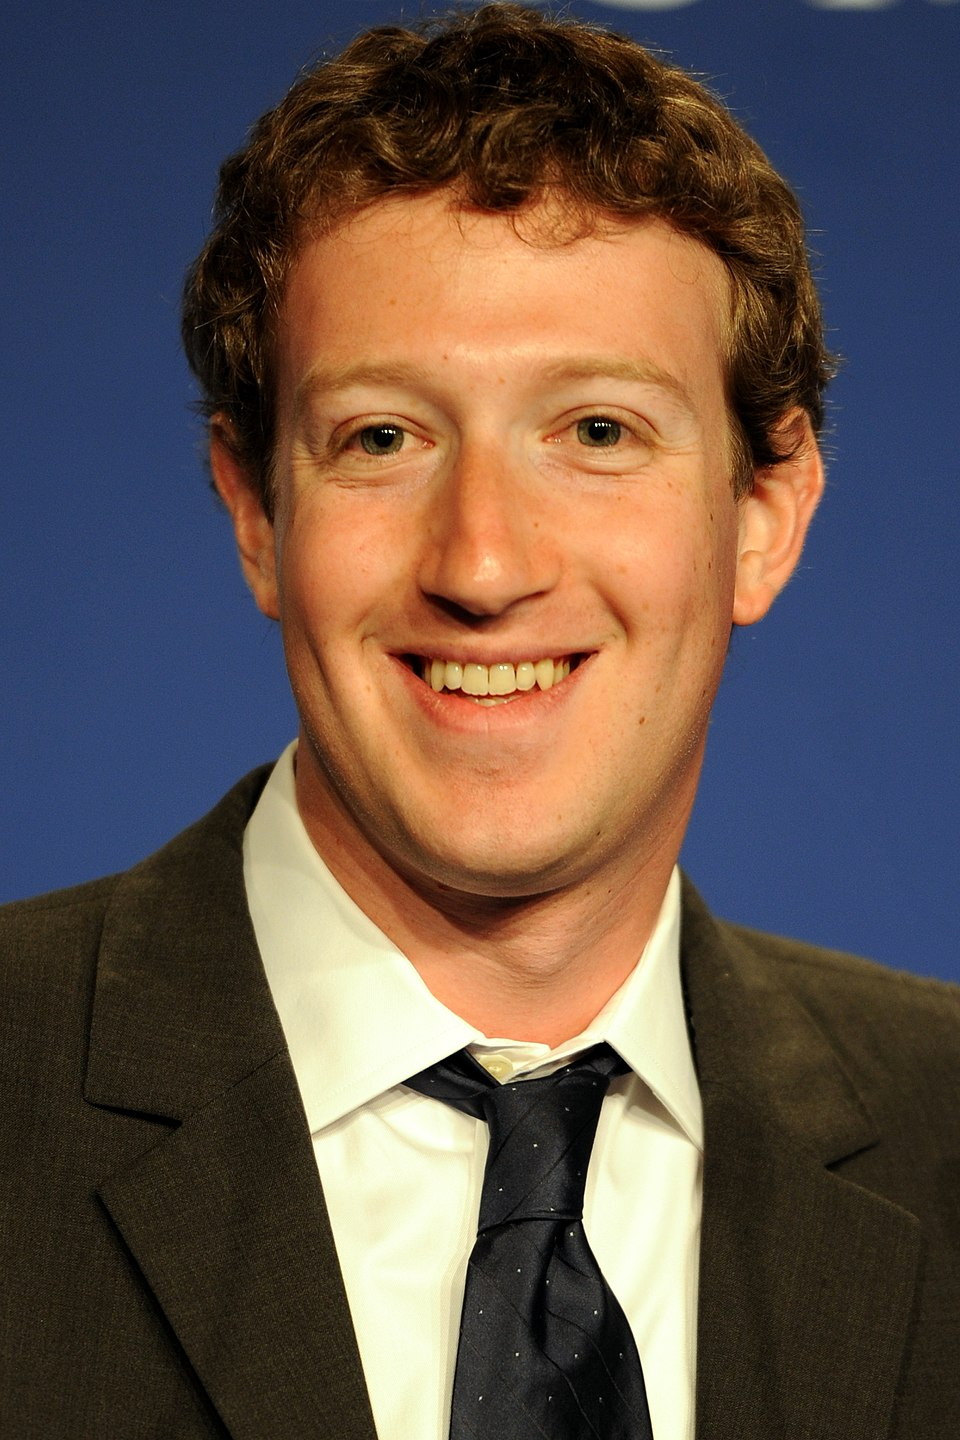
\includegraphics[width=3.4375in,height=4.30208in]{images/03-2025-08-19_20/03-mark_zuckenberg.jpg} & 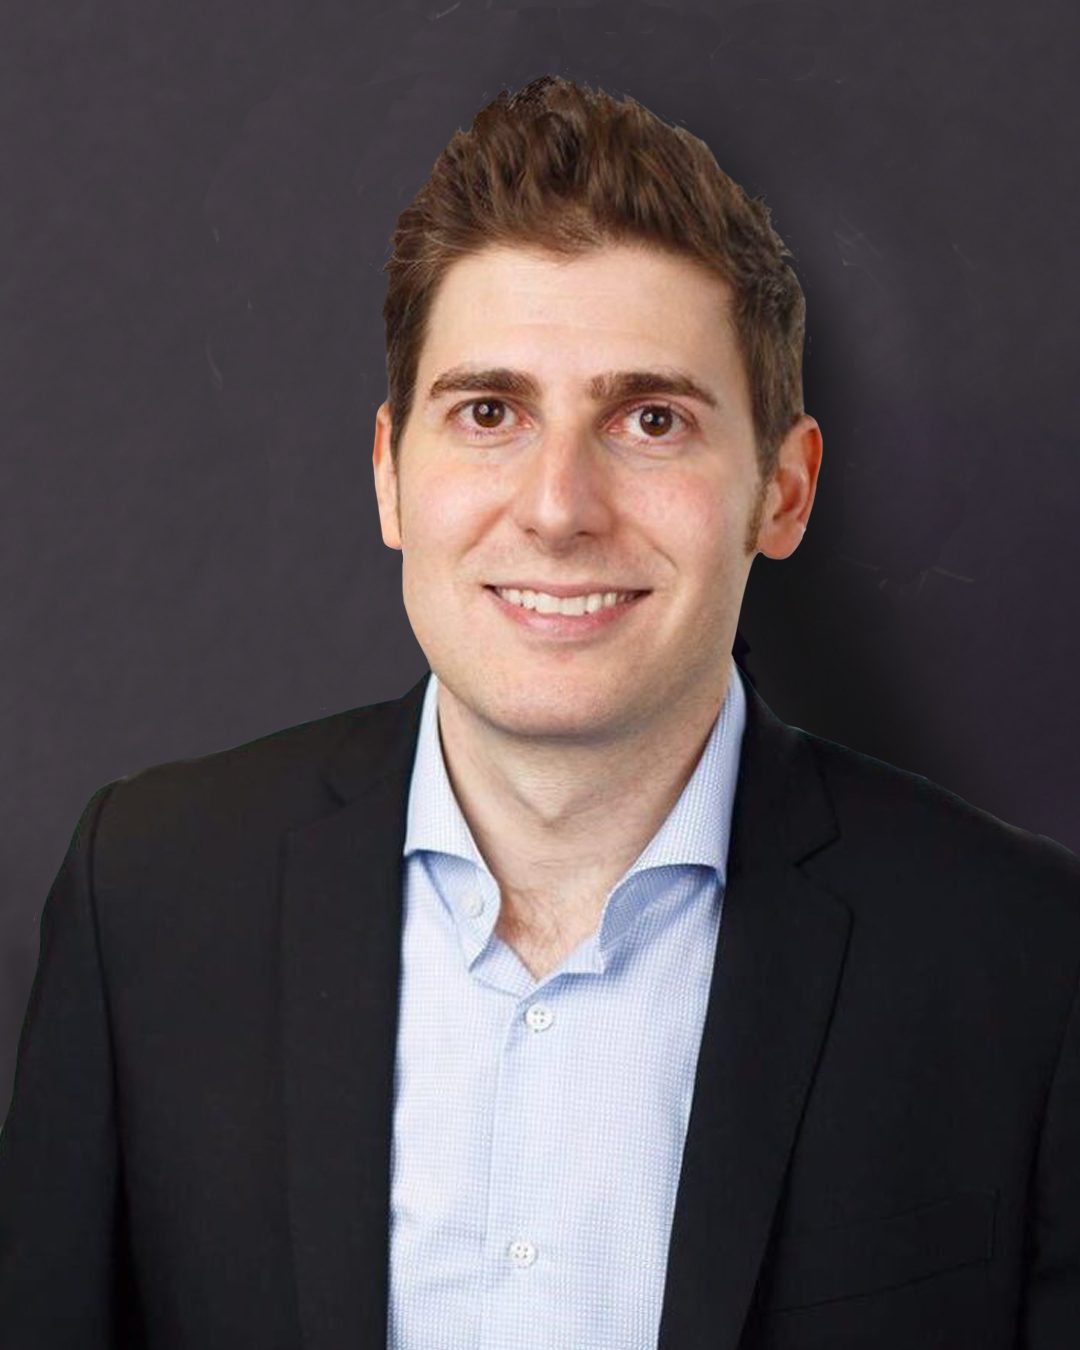
\includegraphics[width=3.95833in,height=\textheight]{images/03-2025-08-19_20/04-eduardo_saverin.jpg} \\
\end{longtable}

\begin{longtable}[]{@{}
  >{\raggedright\arraybackslash}p{(\columnwidth - 6\tabcolsep) * \real{0.2297}}
  >{\raggedright\arraybackslash}p{(\columnwidth - 6\tabcolsep) * \real{0.2297}}
  >{\raggedright\arraybackslash}p{(\columnwidth - 6\tabcolsep) * \real{0.2297}}
  >{\raggedright\arraybackslash}p{(\columnwidth - 6\tabcolsep) * \real{0.3108}}@{}}
\toprule\noalign{}
\begin{minipage}[b]{\linewidth}\raggedright
Data (Estim)
\end{minipage} & \begin{minipage}[b]{\linewidth}\raggedright
Evento Chave
\end{minipage} & \begin{minipage}[b]{\linewidth}\raggedright
Equity Saverin(Estim)
\end{minipage} & \begin{minipage}[b]{\linewidth}\raggedright
Contexto e Ação
\end{minipage} \\
\midrule\noalign{}
\endhead
\bottomrule\noalign{}
\endlastfoot
Fevereiro de 2004 & Fundação do Facebook & 30\% a 34\% & \textbf{Eduardo Saverin} investe \textbf{US\$ 15 mil} para ajudar a fundar a empresa. \textbf{Sua participação é a maior entre os sócios}, atrás apenas de \textbf{Mark Zuckerberg}. \\
Metade de 2004 & Mudança para Palo Alto & \textless{} 30\% & Desentendimentos entre Zuckerberg e Saverin. Zuckerberg começa a buscar novos investidores e a estruturar a empresa legalmente para uma nova rodada de investimento. \\
Junho de 2004 & Aporte de Peter Thiel & \textasciitilde20\% a 25\% & \textbf{Peter Thiel} e \textbf{Reid Hoffman} (investidores-anjo) injetam \textbf{US\$ 500 mil} no Facebook. Esta é a primeira rodada de investimento que causa a diluição da participação dos fundadores. \\
Final de 2004 & Reestruturação e Exclusão & \textless{} 10\% & \textbf{Zuckerberg} cria uma \textbf{nova entidade legal} (``Thefacebook, Inc.''), emite novas ações e, de forma controversa, \textbf{dilui a participação de Saverin} a uma porcentagem mínima \textbf{sem seu consentimento}. \\
Maio de 2005 & Rodada de Série A & \textasciitilde10\% & A \textbf{Accel Partners} e o co-fundador da PayPal investem \textbf{US\$ 12,7 milhões} na empresa. \textbf{Ações adicionais são emitidas}, \textbf{diluindo ainda mais todos os fundadores}, incluindo \textbf{Saverin}. \\
Setembro de 2005 & Processo Judicial de Saverin & \textasciitilde10\% & \textbf{Saverin} processa \textbf{Zuckerberg} e o Facebook, alegando que \textbf{foi diluído de forma ilegal} e \textbf{quebra de contrato}. \\
2006 & Rodada de Série B & \textless{} 10\% & \textbf{Accel Partners}, \textbf{Greylock Partners} e outros \textbf{investem US\$ 27,5 milhões}. A diluição continua. \\
2007 & Rodada da Microsoft & \textless{} 5\% & \textbf{A Microsoft investe US\$ 240 milhões}, avaliando o \textbf{Facebook em US\$ 15 bilhões}. A \textbf{emissão de novas ações dilui drasticamente a participação de todos os sócios}. \\
2008 & Acordo com Saverin & \textasciitilde4\% & Saverin e Zuckerberg chegam a um acordo extrajudicial. Os termos exatos não são revelados, mas é noticiado que Saverin recebe uma quantia em dinheiro, suas ações são restauradas, e ele é readmitido como cofundador. \\
Maio de 2012 & IPO do Facebook & \textasciitilde2\% & No momento da \textbf{Oferta Pública Inicial (IPO)}, a participação de Saverin é amplamente divulgada como \textbf{estando em torno de 2\%}. O \textbf{valor de sua fatia é estimado em cerca de US\$ 4 bilhões}. \\
& & & \\
\end{longtable}

\subsection{Exemplos}\label{exemplos}

(Investimento do tipo Seed Capital)

\begin{longtable}[]{@{}
  >{\raggedright\arraybackslash}p{(\columnwidth - 0\tabcolsep) * \real{1.0000}}@{}}
\toprule\noalign{}
\begin{minipage}[b]{\linewidth}\raggedright
EXEMPLO 1 - Você é o único fundador da startup ``\textbf{Tech-Solve}'' e possui 1.000.000 (um mihão) de cotas da empresa, que representam 100\% do \textbf{EQUITY}. Um investidor anjo (seed capital) se interessa em investir. O valuation (valor da empresa antes do investimento) é de \textbf{R\$ 5.000.000,00} . O investidor quer injetar um capital de \textbf{R\$ 1.000.000} na empresa. Para \textbf{não perder a maioria}, qual o \textbf{número máximo de cotas} você pode ceder a ele, considerando que cada cota tem um valor unitário?
\end{minipage} \\
\midrule\noalign{}
\endhead
\bottomrule\noalign{}
\endlastfoot
a) 250.000 cotas \\
b) 200.000 cotas \\
c) 150.000 cotas \\
d) 100.000 cotas \\
\end{longtable}

\subsection{Resolução:}\label{resoluuxe7uxe3o}

O primeiro exemplo trata de um conceito fundamental para qualquer fundador de startup: a diluição do equity. O objetivo é calcular quantas cotas o \textbf{investidor anjo} deve receber para que ele injete \textbf{R\$ 1.000.000} na empresa.

Vamos resolver o exercício passo a passo:

\textbf{1. Calcular o valor da empresa após o aporte (Post-money Valuation):}

\begin{itemize}
\item
  \textbf{Capital Social da empresa (Valuation) pré-aporte}:

  R\$ 5.000.000
\item
  \textbf{Aporte do investidor}:

  R\$ 1.000.000
\item
  \textbf{Capital Social da empresa (Valuation) (pós-aporte)}:

  \$ ( R\$ 5.000.000) + ( R\$ 1.000.000 ) = \textbf{R\$ 6.000.000}
\end{itemize}

\textbf{2. Calcular a participação do investidor (em percentual):}

\begin{itemize}
\item
  A participação do investidor é a porcentagem que o valor do aporte representa no valor da empresa após o aporte.

  \[
  ParticipaçãoInvestidor = (\frac{ R$ 1.000.000}{ R$ 6.000.000}) * 100%
  \]

  \[
  ParticipaçãoInvestidor = \textbf{16,67%}
  \]
\item
  \textbf{Percentual do investidor}: (R\$ 1.000.000 / R\$ 6.000.000) * 100\% = \textbf{16,67\%}
\end{itemize}

\textbf{3. Calcular o total de cotas após o aporte:}

\begin{enumerate}
\def\labelenumi{\Roman{enumi}.}
\item
  Você, como fundador, tem 1.000.000 de cotas, que representam 100\% do valor da empresa antes do aporte.
\item
  Para encontrar o número total de cotas após o aporte, podemos usar a seguinte fórmula:

  \begin{itemize}
  \tightlist
  \item
    \textbf{Total de cotas (pós-aporte)} = (Cotas do fundador / Participação do fundador)
  \end{itemize}
\item
  Como o investidor terá 16,67\%, sua participação será de 100\% - 16,67\% = 83,33\%.
\item
  \textbf{Total de cotas (pós-aporte)} = 1.000.000 / 0,8333 = \textbf{1.200.000 cotas}
\end{enumerate}

\textbf{4. Calcular o número de cotas a serem cedidas ao investidor:}

\begin{enumerate}
\def\labelenumi{\Roman{enumi}.}
\item
  Agora que sabemos o total de cotas e o seu número de cotas (que não muda), podemos calcular quantas cotas o investidor vai receber.
\item
  \textbf{Cotas do investidor} = Total de cotas (pós-aporte) - Cotas do fundador
\item
  \textbf{Cotas do investidor} = 1.200.000 - 1.000.000 = \textbf{200.000 cotas}
\end{enumerate}

\textbf{Resposta correta:}

A alternativa \textbf{b) 200.000 cotas}.

Resumo:

\begin{itemize}
\item
  \textbf{Valor do Aporte:} R\$ 1.000.000
\item
  \textbf{Valuation Pré-Aporte:} R\$ 5.000.000
\item
  \textbf{Cotas Originais do Fundador:} 1.000.000
\end{itemize}

\begin{enumerate}
\def\labelenumi{\arabic{enumi}.}
\item
  \textbf{Valuation Pós-Aporte} = R\$ 5.000.000 + R\$ 1.000.000 = \textbf{R\$ 6.000.000}
\item
  \textbf{Participação do Investidor} = (R\$ 1.000.000 / R\$ 6.000.000) * 100 = \textbf{16,67\%}
\item
  \textbf{Participação do Fundador Pós-Aporte} = 100\% - 16,67\% = \textbf{83,33\%}
\item
  \textbf{Total de Cotas Pós-Aporte} = 1.000.000 / 0,8333 = \textbf{1.200.000 cotas}
\item
  \textbf{Cotas Cedidas ao Investidor} = 1.200.000 - 1.000.000 = \textbf{200.000 cotas}
\end{enumerate}

Você pode continuar a praticar com os próximos exercícios se quiser! Eles vão aprofundar a sua compreensão sobre como a diluição e o controle de propriedade funcionam ao longo do tempo.

\subsection{\texorpdfstring{\textbf{Exercício 2: Aporte Venture Capital (Série A)}}{Exercício 2: Aporte Venture Capital (Série A)}}\label{exercuxedcio-2-aporte-venture-capital-suxe9rie-a}

\begin{longtable}[]{@{}
  >{\raggedright\arraybackslash}p{(\columnwidth - 0\tabcolsep) * \real{1.0000}}@{}}
\toprule\noalign{}
\endhead
\bottomrule\noalign{}
\endlastfoot
Exercício 2 - Após o aporte inicial, sua startup ``Tech-Solve'' tem agora 1.200.000 cotas e um Capital Social (valuation) de R\$ 10.000.000. Você ainda detém 1.000.000 de cotas. Um fundo de Venture Capital se propõe a investir R\$ 3.000.000. Para que você mantenha o controle majoritário da empresa (mais de 50\% das cotas após o aporte), qual o número máximo de cotas que você pode ceder neste novo round? \\
a) 500.000 cotas \\
b) 428.571 cotas \\
c) 300.000 cotas \\
d) 250.000 cotas \\
\end{longtable}

\subsection{\texorpdfstring{\textbf{Exercício 3:} Aporte Growth Capital (Série B)}{Exercício 3: Aporte Growth Capital (Série B)}}\label{exercuxedcio-3-aporte-growth-capital-suxe9rie-b}

\begin{longtable}[]{@{}
  >{\raggedright\arraybackslash}p{(\columnwidth - 0\tabcolsep) * \real{1.0000}}@{}}
\toprule\noalign{}
\endhead
\bottomrule\noalign{}
\endlastfoot
Exercício 3 - ``Tech-Solve'' cresceu e agora tem um valuation de R\$ 50.000.000, com um total de 1.700.000 cotas. Você, como fundador, tem 1.000.000 cotas. Um novo investidor de Growth Capital quer injetar R\$ 15.000.000. Qual o percentual de diluição que você sofrerá após este novo aporte, assumindo que você ceda cotas suficientes para o investimento? \\
a) 23,08\% \\
b) 18,75\% \\
c) 20,00\% \\
d) 25,00\% \\
\end{longtable}

\subsection{Exercício 4: Cenário de Múltiplos Investidores}\label{exercuxedcio-4-cenuxe1rio-de-muxfaltiplos-investidores}

\begin{longtable}[]{@{}
  >{\raggedright\arraybackslash}p{(\columnwidth - 0\tabcolsep) * \real{1.0000}}@{}}
\toprule\noalign{}
\endhead
\bottomrule\noalign{}
\endlastfoot
Exercício 4 - ``Tech-Solve'' agora tem 1.000.000 de cotas originais, um investidor A com 200.000 cotas e um investidor B com 500.000 cotas. Sua participação é de 1.000.000 de cotas. A empresa está avaliada em R\$ 20.000.000. Um novo investidor quer comprar 10\% da empresa. Quantas cotas ele deve receber, e qual será sua nova participação percentual na empresa? \\
a) 150.000 cotas; 8,8\% \\
b) 200.000 cotas; 10,0\% \\
c) 190.000 cotas; 9,5\% \\
d) 170.000 cotas; 8,5\% \\
\end{longtable}

\subsection{Exercício 5: Protegendo a Maioria}\label{exercuxedcio-5-protegendo-a-maioria}

\begin{longtable}[]{@{}
  >{\raggedright\arraybackslash}p{(\columnwidth - 0\tabcolsep) * \real{1.0000}}@{}}
\toprule\noalign{}
\endhead
\bottomrule\noalign{}
\endlastfoot
Exercício 5 - Considere que, após todos os aportes (do Exercício 1 ao 4), você ainda deseja manter o controle majoritário da sua startup. O investidor A tem 200.000 cotas e o investidor B tem 500.000 cotas. No último aporte, o investidor C recebeu 190.000 cotas. Você começou com 1.000.000 de cotas. Qual a sua participação percentual atual na empresa, e você ainda tem a maioria? \\
a) 50,0\% - Não tem a maioria \\
b) 51,5\% - Tem a maioria \\
c) 48,0\% - Não tem a maioria \\
d) 49,5\% - Não tem a maioria \\
\end{longtable}

\section{Respostas dos exercícios}\label{respostas-dos-exercuxedcios}

\begin{longtable}[]{@{}ll@{}}
\toprule\noalign{}
\endhead
\bottomrule\noalign{}
\endlastfoot
Exercício & Resposta \\
1 Modelo & b \\
2 & c \\
3 & a \\
4 & c \\
5 & b \\
\end{longtable}

\section{Referências}\label{referuxeancias-1}

ROSSETTI, José Paschoal; ANDRADE, Adriana. \emph{Governança Corporativa: Fundamentos, Desenvolvimento e Tendências}. São Paulo: Atlas, 7. ed., 2014. p.~s.p.

\chapter{Governança Corporativa - Conselhos da Empresa}\label{governanuxe7a-corporativa---conselhos-da-empresa}

\subsubsection*{26/08/2025 - Campus Marquês}\label{campus-marquuxeas-3}
\addcontentsline{toc}{subsubsection}{26/08/2025 - Campus Marquês}

\subsubsection*{27/08/2025 - Campus Chácara}\label{campus-chuxe1cara-3}
\addcontentsline{toc}{subsubsection}{27/08/2025 - Campus Chácara}

\section{Referências}\label{referuxeancias-2}

ROSSETTI, José Paschoal; ANDRADE, Adriana. \emph{Governança Corporativa: Fundamentos, Desenvolvimento e Tendências}. São Paulo: Atlas, 7. ed., 2014. p.~s.p.

\chapter{Governança Corporativa - C Level e Diretorias}\label{governanuxe7a-corporativa---c-level-e-diretorias}

\subsubsection*{02/09/2025 - Campus Marquês}\label{campus-marquuxeas-4}
\addcontentsline{toc}{subsubsection}{02/09/2025 - Campus Marquês}

\subsubsection*{03/09/2025 - Campus Chácara}\label{campus-chuxe1cara-4}
\addcontentsline{toc}{subsubsection}{03/09/2025 - Campus Chácara}

\section{Referências}\label{referuxeancias-3}

ROSSETTI, José Paschoal; ANDRADE, Adriana. \emph{Governança Corporativa: Fundamentos, Desenvolvimento e Tendências}. São Paulo: Atlas, 7. ed., 2014. p.~s.p.

\chapter{Governança da Informação - Diretoria de Informática}\label{governanuxe7a-da-informauxe7uxe3o---diretoria-de-informuxe1tica}

\subsubsection*{09/09/2025 - Campus Marquês}\label{campus-marquuxeas-5}
\addcontentsline{toc}{subsubsection}{09/09/2025 - Campus Marquês}

\subsubsection*{10/09/2025 - Campus Chácara}\label{campus-chuxe1cara-5}
\addcontentsline{toc}{subsubsection}{10/09/2025 - Campus Chácara}

\section{Referências}\label{referuxeancias-4}

ROSSETTI, José Paschoal; ANDRADE, Adriana. \emph{Governança Corporativa: Fundamentos, Desenvolvimento e Tendências}. São Paulo: Atlas, 7. ed., 2014. p.~s.p.

\chapter{Governança da Informação - Modelo COBIT 5.0}\label{governanuxe7a-da-informauxe7uxe3o---modelo-cobit-5.0}

\subsubsection*{23/09/2025 - Campus Marquês}\label{campus-marquuxeas-6}
\addcontentsline{toc}{subsubsection}{23/09/2025 - Campus Marquês}

\subsubsection*{24/09/2025 - Campus Chácara}\label{campus-chuxe1cara-6}
\addcontentsline{toc}{subsubsection}{24/09/2025 - Campus Chácara}

\chapter{Governança da Informação - COBIT 5.0 - Os 5 Princípios}\label{governanuxe7a-da-informauxe7uxe3o---cobit-5.0---os-5-princuxedpios}

\subsubsection*{30/09/2025 - Campus Marquês}\label{campus-marquuxeas-7}
\addcontentsline{toc}{subsubsection}{30/09/2025 - Campus Marquês}

\subsubsection*{01/10/2025 - Campus Chácara}\label{campus-chuxe1cara-7}
\addcontentsline{toc}{subsubsection}{01/10/2025 - Campus Chácara}

\chapter{Governança da Informação - COBIT 5.0 - Os 7 Habilitadores}\label{governanuxe7a-da-informauxe7uxe3o---cobit-5.0---os-7-habilitadores}

\subsubsection*{07/10/2025 - Campus Marquês}\label{campus-marquuxeas-8}
\addcontentsline{toc}{subsubsection}{07/10/2025 - Campus Marquês}

\subsubsection*{08/10/2025 - Campus Chácara}\label{campus-chuxe1cara-8}
\addcontentsline{toc}{subsubsection}{08/10/2025 - Campus Chácara}

\chapter{Governança da Informação - COBIT 5.0 - Implantação}\label{governanuxe7a-da-informauxe7uxe3o---cobit-5.0---implantauxe7uxe3o}

\subsubsection*{14/10/2025 - Campus Marquês}\label{campus-marquuxeas-9}
\addcontentsline{toc}{subsubsection}{14/10/2025 - Campus Marquês}

\subsubsection*{15/10/2025 - Campus Chácara}\label{campus-chuxe1cara-9}
\addcontentsline{toc}{subsubsection}{15/10/2025 - Campus Chácara}

\chapter{Governança da Informação - COBIT 2019 - O que mudou em relação ao 5.0}\label{governanuxe7a-da-informauxe7uxe3o---cobit-2019---o-que-mudou-em-relauxe7uxe3o-ao-5.0}

\subsubsection*{21/10/2025 - Campus Marquês}\label{campus-marquuxeas-10}
\addcontentsline{toc}{subsubsection}{21/10/2025 - Campus Marquês}

\subsubsection*{22/10/2025 - Campus Chácara}\label{campus-chuxe1cara-10}
\addcontentsline{toc}{subsubsection}{22/10/2025 - Campus Chácara}

\chapter{Governança da Informação - Revisão}\label{governanuxe7a-da-informauxe7uxe3o---revisuxe3o}

\subsubsection*{28/10/2025 - Campus Marquês}\label{campus-marquuxeas-11}
\addcontentsline{toc}{subsubsection}{28/10/2025 - Campus Marquês}

\subsubsection*{29/10/2025 - Campus Chácara}\label{campus-chuxe1cara-11}
\addcontentsline{toc}{subsubsection}{29/10/2025 - Campus Chácara}

  \bibliography{book.bib}

\end{document}
